\documentclass[]{final_report}
\usepackage{graphicx}
\graphicspath{ {./images/} }
\usepackage{hyperref}
\usepackage{amssymb}
\usepackage{amsmath}

%%%%%%%%%%%%%%%%%%%%%%
%%% Input project details
\def\studentname{Cougar Tasker}
\def\reportyear{2023-24}
\def\projecttitle{Resourceful Robots}
\def\supervisorname{Dr. Anand Subramoney}
\def\degree{MSci (Hons) in Computer Science (Artificial Intelligence)}
\def\fullOrHalfUnit{Full Unit} % indicate if you are doing the project as a Full Unit or Half Unit
\def\finalOrInterim{Interim Report} % indicate if this document is your Final Report or Interim Report

\begin{document}

\maketitle

%%%%%%%%%%%%%%%%%%%%%%
%%% Declaration

\chapter*{Declaration}

This report has been prepared on the basis of my own work. Where other published and unpublished source materials have been used, these have been acknowledged.

\vskip3em

Word Count: 

\vskip3em

Student Name: \studentname

\vskip3em

Date of Submission: 

\vskip3em

Signature:

\newpage

%%%%%%%%%%%%%%%%%%%%%%
%%% Table of Contents
\tableofcontents\pdfbookmark[0]{Table of Contents}{toc}\newpage

%%%%%%%%%%%%%%%%%%%%%%
%%% Your Abstract here

\begin{abstract}

This document serves as a layout and formatting template for your project report. It does not tell you how to write it, or what it should contain. It explains how it should be formatted and typeset. Please refer to your project booklet for information about report sizes, contents and rules.

\textbf{\textit{NOTE: in your report, you should replace this with an appropriate Abstract for your project report.}}

\end{abstract}
\newpage

%%%%%%%%%%%%%%%%%%%%%%
%%% Project Spec

\chapter*{Project Specification}
\addcontentsline{toc}{chapter}{Project Specification}
Your project specification goes here.

%%%%%%%%%%%%%%%%%%%%%%
%%% Introduction
\chapter{Introduction}

The project report is a very important part of your project and its preparation and presentation should be of extremely high quality. Remember that a significant portion of the marks for your project are awarded for this report. 

The format of the final report is fixed by the template of this document and the Department of Computer Science suggests its usage. 

While this may sound like a rather prescriptive approach to report writing, it is introduced for the following reasons:
\begin{enumerate}
 \item The template allows students to focus on the critical task of producing clear and concise content, instead of being distracted by font settings and paragraph spacing. 
 \item By providing a comprehensive template the Department benefits from a consistent and professional look to its internal project reports.
\end{enumerate}

The remainder of this document briefly outlines the main components and their usage.

A \textbf{final project report} is approximately 15,000 words and must include a word count. It is acceptable to have other material in appendixes.  
Your \textbf{interim report} for the December Review meeting, even if it is a collection of reports, should have a total word count of about 5,000 words. 
This should summarise the work you have done so far, with sections on the theory you have learnt and the code that you have written.

Also remember that any details of report content and submission rules, as well as other deliverables, are defined in the project booklet

\section{How to use this template}

The simplest way to get started with your report is to save a copy of this document. 
First change the values for the initial document definitions such as \verb|studentname| and \verb|reportyear| to match your details.
Delete the unneeded sections and start adding your own sections using the styles provided.
Before submission, remember to fill in the Declaration section fields.

\chapter{Markov Decision Processes} 

Markov Decision Processes (MDP) provide a mathematical formalisation of decision-making problems. Markov Decision Processes provide the foundation for reinforcement learning (RL). This is because MDPs distil the fundamental parts of decision-making, allowing RL techniques built upon MDPs to generalise to learning in the real world and across different domains such as finance and robotics. 

As a formal mathematical framework, MDPs allow us to derive and prove statements about our RL methods built upon them. An important example of this is that we can prove that Q-learning (an RL technique explained in chapter~\ref{chap:q-learning}) will converge to the true Q-values as long as each Action-State pair is visited infinitely often. \cite{watkins1992q}. Furthermore, MDPs allow us to reason about problems with uncertainty allowing RL agents to account for randomness in their environment. 

The standardisation of decision-making problems as MDPs allows for a uniform definition of optimality with the value functions. MDPs give a basis for assessing the performance of RL algorithms, facilitating like-for-like comparisons for different RL approaches. 


\section{Markov Property}

The Markov property is that the future state of a Markov system only depends on the current state of the system. In other words, if we have a system that follows the Markov property, then the history preceding the current configuration of the system will not influence the following state.

To put the Markov property formally $S_t$ represents the state at some time $t$. $S_t$ represents the outcome of some random variable. Then the Markov property would hold if and only if:

$$\Pr(S_{c+1}\ |\ S_{c},S_{c-1},\dots,S_0) = \Pr(S_{c+1}\ |\ S_{c})$$

This definition demonstrates how the Markov property can hold in non-deterministic, stochastic processes. It also shows that predictions that are only based on the current state are just as good as those that record the history in a Markov process. The sequence of events in this definition, $S_t$, is called a Markov Chain\cite{meyn2012markov}.

\newpage
\section{Extending Markov Chains}

Markov Decision Processes extend Markov Chain's in two important ways. Firstly MDPs introduce decision-making through actions. Each state in an MDP has a set of available actions in that state. In each state, an action is required to transition to the next state; this action with the current state can affect what the following state will be. Secondly, MDPs introduce a reward value. The reward is determined from the current state and action; it is produced simultaneously with the following state.

A formal definition of a Markov Decision Process is a tuple $(\mathcal{S},\mathcal{A}_s,p)$ where:
\begin{itemize}
  \item $\mathcal{S}$ defines the set of all states
  \item $\mathcal{A}_s$ defines the set of available actions in state $s$
  \item $p$ defines the relationship between states, actions and rewards: \\
  $p(s',r\ |\ s,a) \doteq \Pr(S_{t+1} = s', R_{t+1} = r | S_t = s, A_t = a)\cite{sutton2018reinforcement}$
  \begin{itemize}
    \item $s, s' \in \mathcal{S}$, $a \in \mathcal{A}_s$ and $r \in \mathbb{R}$
    \item $p: \mathcal{S} \times \mathbb{R} \times \mathcal{S} \times \mathcal{A} \rightarrow [0,1]$
  \end{itemize}
\end{itemize}

The function $p$ is an integral part of this definition; it fully describes how the system will evolve. We call this function the dynamics of the MDP. What this definition does not describe is how actions are chosen. This decision-making is done by an entity called an agent. For our purposes, the agent will have complete visibility as to the current state of the MDP. However, like most real-world situations, our agent will not have any a priori knowledge of the dynamics. 

\begin{figure}[h]
  \centering
  \fboxsep 2mm
  \framebox{
    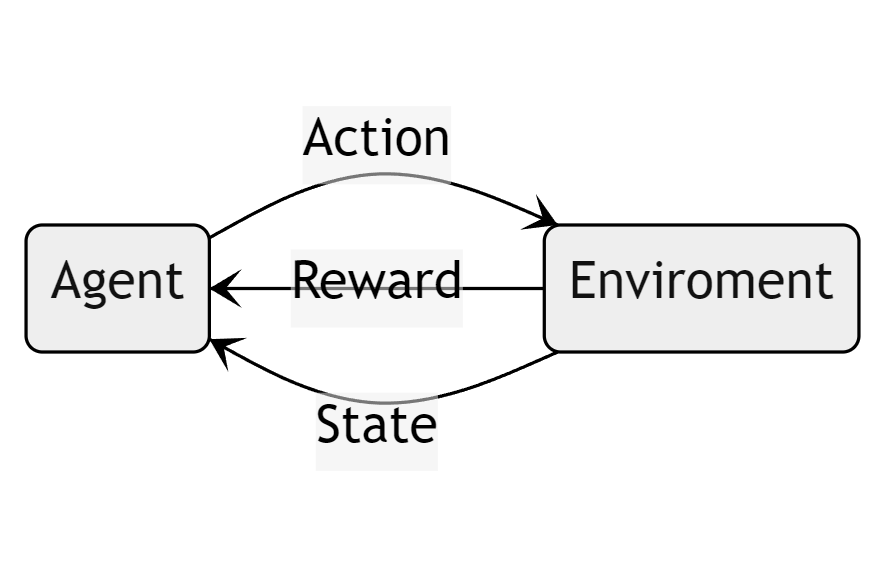
\includegraphics[width=6cm]{agent-enviroment} 
  }
  \caption{\label{fig:agent-enviroment} The agent-environment interface}
\end{figure} 
% stateDiagram-v2
%     direction LR
%     a : Agent
%     e : Enviroment
    
%     a --> e : Action
%     e --> a : Reward
%     e --> a : State

The agent comprises the entire decision-making entity in an MDP; anything unknown or not wholly under the agent's control is called the agent's environment. In the context of reinforcement learning, the environment is essentially the dynamics of the MDP. Figure~\ref{fig:agent-enviroment} demonstrates how the agent and environments affect each other in an MDP. 

\label{policy-informal-definition}
For learning agents, we wish to improve the agent's behaviour over time. For this purpose, we introduce a policy $\pi$. This policy defines the action chosen by an agent under a particular state. The policy can be represented with a lookup table like in Q-learning\ref{chap:q-learning} or a more complex process such as deep Q-learning. A policy like this is not hard-coded, allowing the agent to update the policy based on the information the agent learns from the environment. 



\chapter{Policy and Value functions}

After each action, a reward is received. It follows that the goal of an agent should be to choose the actions to maximise these reward signals received. Following the Markov principle and the definition of an MDP, this reward only depends on the current state and the action chosen. Consequently, being in some states and performing some actions are more valuable to the agent than other states and actions. We can define value functions: 
\begin{itemize}
  \item $v(s)$ function determines the value of being in a given state
  \item $q(s,a)$ function determines the value of being in a given state and performing a specific action
\end{itemize}
 

% stateDiagram-v2
%     a --> b : R = 0
%     b --> b : R = 100
\begin{figure}[h]
  \centering
  \fboxsep 2mm
  \framebox{
    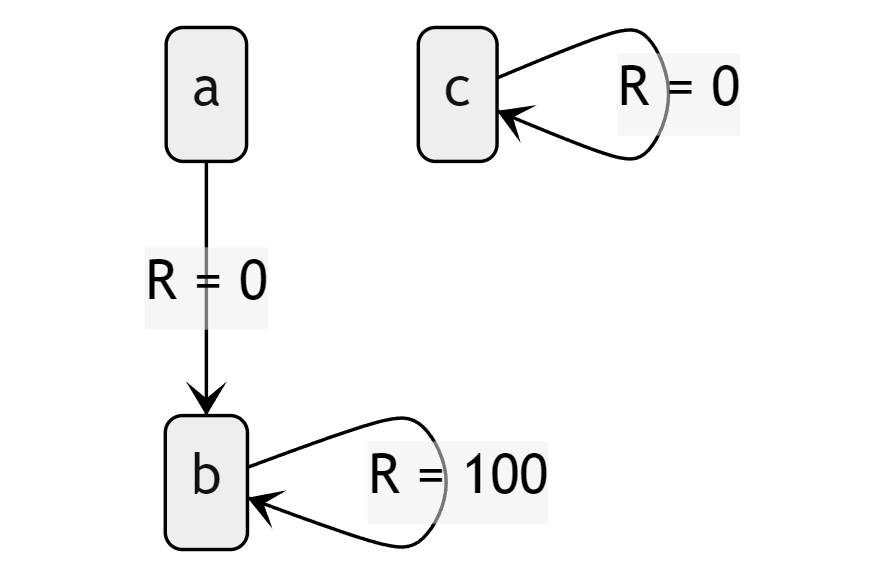
\includegraphics[width=6cm]{reward-example} 
  }
  \caption{\label{fig:reward-example} An example of transitive value of states $v(b) > v(a) > v(c)$}
\end{figure} 

Intuitively, the value of being in a state is more than only its immediate reward that might be found from performing actions in that state. It is also related to the potential future reward that might be achieved in the reachable subsequent states. This can be demonstrated with two states $a$, and $b$, where there is a large reward at $b$ and the only way to reach $b$ is through $a$ then being at $a$ is also valuable regardless of the reward available at $a$. However, $a$ can be considered less valuable than $b$, because it always requires more steps to achieve the reward from $a$ than at $b$. To account for preferring more immediate rewards, the value function should also discount future value with a parameter $\gamma$. 


These value functions go hand in hand with an agent's policy; a good policy maximises being in valuable states and performing valuable actions. On the other side of the coin, the value is determined by the subsequent states and rewards, which are in part determined by the actions the policy selects. Basing the policy on the value function gives the value function's definition impact over that agent's decision-making, in particular, the discount rate ($\gamma$). With high discount rates $\gamma \approx 1$ the agent can be far-sighted and ignore short-term high-reward actions available to it and take longer to learn. With low discount rates $\gamma \approx 0$, the agent can be short-sighted, ignoring the potential long-term benefits of certain actions.

While the policy is informally described at the end of chapter~\ref{policy-informal-definition}, a formal definition of a policy ($\pi$) is the probability distribution of an agent picking a given action in a given state:
 $$\pi(a \ |\ s) \doteq \Pr(A_t = a | S_t = s)$$
Where $s \in \mathcal{S}$ and $a \in \mathcal{A}_s$. This definition shows how the policy can be stochastic. A stochastic policy can be beneficial in many ways, such as breaking ties where multiple actions are equally good and choosing between when to explore more or seek rewards. 

\section{optimal policy/value function via the Bellman equation}

With a known policy and dynamics, the future state can be wholly determined, allowing for a complete mathematical definition of the value functions under a given policy that describes our above intuitions. for the state-value function ($v$) and action-value function ($q$) under a policy $\pi$ we have the formulas:

$$q_\pi(s,a) \doteq \sum_{s',r}p(s',r\ |\ s, a)[r + \gamma v_\pi(s')]$$
$$v_\pi(s) \doteq \sum_a \pi(a\ |\ s) q_\pi(s,a)$$

These value functions are defined recursively in terms of each other; these definitions can be unrolled to only be in terms of themselves. The unrolled form of the state-value function is known as the Bellman equation. These equations are named Richard Bellman, who, in the process of developing the field of dynamic programming, created them\cite{bellman1957}.   

These functions demonstrate the intertwined relationships between the policy chosen and the value of that state if there is a particularly valuable action $a^\ast$ such that $q_\pi(s,a^\ast)$ is far better than for all other actions. A policy $\pi(a^\ast\ |\ s) = 0$ would hamper the potential value of $s$. Therefore, the value function can be used to compare how well different policies perform. If for policy $\pi_a$ there does not exist another policy $\pi_b$ such that $\pi_b$ has a better value $v_{\pi_b}(s) > v_{\pi_a}(s)$ for all states $s \in \mathcal{S}$ then we can consider this policy $\pi_a$ an optimal policy. There may be many optimal policies; however, we often do not need to distinguish them, so we often denote any optimal policy with $\pi_\ast$. This is because all optimal polices share the same state-value, and by definition action-value, function, we denote these $v_\ast$ and $q_\ast$. The optimal value function $v_\ast$ is known as Bellman optimality equation. These optimal equations can be written formally as:

$$v_\ast(s) \doteq \max_\pi v_\pi(s) $$
$$q_\ast(s,a) \doteq \max_\pi q_\pi(s,a) $$



\section{Finding optimal policies by iteration}\label{iteration-approaches}

Although optimal policies exist, finding them is another matter. The policy search space is potentially infinite so an intelligent method is required. An optimal policy can be extracted from an optimal value function and the dynamics of the MDP; the optimal policy would only select actions that result in the highest value. Finding the optimal value function with the optimal policy is straightforward, but this is a catch-22. The optimal value function must be self-consistent with the Bellman equations. One approach to solving these equations is iteration, for each step moving slightly closer to the optimal solution from an initial guess. 

\subsection{Policy iteration}

In policy iteration, we improve a policy over time until it is optimal. updating a policy like this is only possible because of the policy improvement theorem. This theorem considers if we have a policy $\pi_{\text{old}}$. We are at some state $s$, $\pi_{\text{old}}$ will pick the action $a$ under this state $\pi_{\text{old}}(a\ |\ s) = 1$ what happens if we consider some other action $a'$ but then continue to follow the original policy. Because we continue to follow the original policy, we can use the existing value function $v_{\pi_{\text{old}}}(S_{t+1})$ for the subsequent states. We call this slightly adjusted policy $\pi_{\text{new}}$. by applying the bellman equations and the existing value function then we can recalculate the value at $s$ of $\pi_{\text{new}}$ if this new value is better than the original policy then we know that $\pi_{\text{new}}$ must be as good if not better for all states $s \in \mathcal{S}$ than $\pi_{\text{old}}$ thus $\pi_{\text{new}}$ would be a better policy. 


$$\sum_a \pi_{\text{new}}(a\ |\ s) q_{\pi_{\text{old}}}(s,a) \ge v_{\pi_{\text{old}}}(s) \Rightarrow  \pi_{\text{new}} \ge \pi_{\text{old}}$$

For some policy $\pi$ you can apply this policy improvement theorem for every state and action in the MDP. This approach of comparing all actions over all states is called policy improvement. This policy improvement step can be applied iteratively until the policy stops improving. If the policy does not improve over this policy improvement step, then all of the actions are optimal, and this policy is optimal

Although this policy improvement sounds computationally expensive, each state can be considered simultaneously and with a shared base policy, in each iteration, the state-value function is the same; caching this removes redundant calculations. Calculating the value function is improved by using an iterative approach and utilising the previous value function as a launching point.  


\subsection{Value iteration}


**Downside to policy**: each iteration may require multiple sweeps of the state space, although in practice if often doesn't need many iterations


in value iteration there is only one step, the policy is not explicitly defined and updated instead the policy updates implicitly as the value function converges, the policy is to pick whatever action produces the largest value. 

finally the policy is extracted from the value table as the action that maximises the cumulative reward with the value table and the dynamics function 





\chapter{Q-learning}\label{chap:q-learning}

-- the iteration approaches are great but they require knowledge of the dynamics that are not necessarily possible in all cases \ref{iteration-approaches}

-- on policy vs off policy
\chapter{Page Layout \& Size}

The page size and margins have been set in this document. These should not be changed or adjusted. 

In addition, page headers and footers have been included. They will be automatically filled in, so do not attempt to change their contents.

\chapter{Headings}

Your report will be structured as a collection of numbered sections at different levels of detail. For example, the heading to this section is a first-level heading and has been defined with a particular set of font and spacing characteristics. At the start of a new section, you need to select the appropriate \LaTeX{} command, \verb|\chapter| in this case.
\section{Second Level Headings}
Second level headings, like this one, are created by using the command \verb|\section|.
\subsection{Third Level Headings}
The heading for this subsection is a third level heading, which is obtained by using command \verb|\subsection|. In general, it is unlikely that fourth of fifth level headings will be required in your final report. Indeed it is more likely that if you do find yourself needing them, then your document structure is probably not ideal. So, try to stick to these three levels.
\section{A Word on Numbering}
You will notice that the main section headings in this document are all numbered in a hierarchical fashion. You don't have to worry about the numbering. It is all automatic as it has been built into the heading styles. Each time you create a new heading by selecting the appropriate style, the correct number will be assigned. 


\chapter{Presentation Issues}

\section{Figures, Charts and Tables}

Most final reports will contain a mixture of figures and charts along with the main body of text. The figure caption should appear directly after the figure as seen in Figure~\ref{fig:logo} whereas a table caption should appear directly above the table. Figures, charts and tables should always be centered horizontally. 

\begin{figure}[h]
\centering
\fboxsep 2mm
\framebox{
	
\includegraphics[width=6cm]{logo} 
}
\caption{\label{fig:logo} Logo of RHUL.}
\end{figure} 

\section{Source Code}

If you wish to print a short excerpt of your source code,  ensure that you are using a fixed-width sans-serif font such as the Courier font. By using the \verb|verbatim| environment your code will be properly indented and will appear as follows:

\begin{verbatim}
static public void main(String[] args) {
  try  {
    UIManager.setLookAndFeel(UIManager.getSystemLookAndFeelClassName());
  }
  catch(Exception e) {
    e.printStackTrace();
  }
  new WelcomeApp();
} 
\end{verbatim}

\chapter{References}

Use one consistent system for citing works in the body of your report. Several such systems are in common use in textbooks and in conference and journal papers. Ensure that any works you cite are listed in the references section, and vice versa. 

\chapter{Project Information and Rules}

The details about how your project will be assessed, as well as the rules you must follow for this final project report, are detailed in the project booklet.

\textbf{You must read that document and strictly follow it.}


%%%% ADD YOUR BIBLIOGRAPHY HERE
\newpage

\bibliographystyle{IEEEtran}
\bibliography{refrences}
\addcontentsline{toc}{chapter}{Bibliography}
\label{endpage}



\end{document}

\end{article}
